%% ------------------------------------------------------------------------- %%
\chapter{Introdução}
\label{cap:introducao}

  O alinhamento espacial ou geométrico entre duas imagens - a imagem
\textbf{Referência} e a \textbf{Alvo} - da mesma cena é um problema clássico de
visão computacional, chamado de \textbf{Registro de Imagens}. O registro
determina um mapeamento pixel a pixel entre duas imagens, criando uma função de
transformação que leva uma das imagens para o espaço geométrico da outra,
atenuando deformações presentes nas imagens. Essas deformações são criadas por
aquisições em horários diferentes, utilização de sensores diferentes ou
mudanças na posição do sensor.

  O registro é aplicado em imagens médicas com várias finalidades, como por
exemplo: (i) na junção de informações de imagens de diferentes modalidades,
como a sobreposição de imagens de ressonância magnética com imagens de raio-x;
(ii) estudos envolvendo atlas anatómicos, onde cada paciente do estudo tem seus
dados registrados para um modelo de estudo; (iii) corrigir diferenças de
imagens de pré- e pós-operatório, causadas por movimentações do paciente e por
movimentação de tecido mole, como a movimentação do pulmão na respiração.

  Os algoritmos de registro são categorizados baseando-se na natureza da
transformação usada para alinhar as imagens. Os \textbf{Algoritmos de Registro
Rígido} definem o primeiro grupo, onde estão os algoritmos que usam
transformações rigidas, usadas para corrigir deformações simples. Esses
algoritmos modelam a função de registro com uma combinação de rotações,
translações, mudanças de escala ou cisalhamentos. Esse tipo de modelagem não
é sulficiente para corrigir movimentações fisiológicas mais complexas, como
as resultantes do batimento do coração ou do movimento respiratório. Para tal,
os \textbf{Algoritmos de Registro Não-Rígido} são utilizados nesse caso. Esses
algoritmos utilizam transformações não lineares para modelar a deformaçãyo
presente nas imagens. O fluxo óptico ou a utilização de equações de dinâmica de
fluidos para aproximar a transformação são exemplos de soluções para casos
não-rigidos. O estudo se foca nos registros não-rigidos.

  Um dos algoritmos mais utilizados pela comunidade cientifica para resolver
casos de registro não-rigidos é o \textbf{Thin Plate Splies} (TPS). O TPS
modela a deformação presente nas imagens como uma deformação aplicada a uma
chapa fina de metal, utilizando pontos de controle escolhidos nas imagens
como parâmetro para deformar a chapa. Porém o tempo de execução do TPS é alto,
crescendo muito conforme o número de pontos de controle aumentam
\cite{zitova2003image}.

  Logo o TPS se beneficia de algum tipo de aceleração. O principal objetivo do
trabalho é apresentar uma implementação do TPS para o modelo \textit{Single
Instruction, Multiple Data} \cite{patterson2013computer}, modelo esse adotado
pelas Unidades de Processamento Gráfico (GPU). Chamaremos de mapeamento para GPU
essa implementação nesse trabalho. A escolha das GPUs como hardware para a
execução do processo de registro se deve pela sua grande capacidade de
processamento atrelada ao baixo custo do processamento.
%% ------------------------------------------------------------------------- %%
\section{Trabalhos Relacionados}
\label{sec:trabalhosRelacionados}

\subsection{GPGPU}

  De acordo com o levantamento realizado por \cite{owens2007survey}, a partir do
começo dos anos 2000 o contexto GPU sofreu duas mudanças: (i) a capacidade de
processamento teórico das GPUs ultrapssou o das CPUs; (ii) mudanças no hardware
que promoveram a criação de rotinas programáveis pelo usuário. Essas duas
mudanças impulsionaram a pesquisa na área de GPGPU, em especial na criação de
melhores métodos para a programação em GPU. Antes do desenvolvimento de
linguagens de alto nivel para GPU, o problema em questão era mapeado para
chamadas de primitivas gráficas.

  Foi também no começo dos anos 2000 que as linguagens de alto nível para GPU,
chamadas na literatura de \textit{Shading Languages}, começaram a ser
desenvolvidas. Alguns exemplos são \textbf{CG} e \textbf{OpenVIDIA},
introduzidas respectivamente por \cite{mark2003cg} e \cite{fung2005openvidia},
baseadas na sintaxe da linguagem C. As chamadas de alto nivel dessas linguagens
são traduzidas para chamadas de API gráficas, como o \textbf{OpenGL} ou
\textbf{DirectX}, que por fim executam o código na GPU.

  Ao realizar essa tradução direta entre o código escrito e chamadas de API
gráficas as linguagens fazem com que o programador seja obrigado a representar
seus dados como pedaços do  \textit{pipeline} gráfico, como vertices, fragmentos
ou texturas. Em 2004 uma extensão da linguagem C, chamada de \textit{Brook},
foi apresentada por \cite{buck2004brook}. O \textit{Brook} realiza um mapeamento
mais frouxo entre o código escrito pelo programador e as chamadas das API,
introduzindo um nivel de abstração a mais entre o código e as API. Essa
abstração é chamada de \textit{Stream Programming Model}, onde a memória da GPU
é modelada como um bloco n-dimensional de dados a serem operados e o código a
ser executado na GPU é mantido em uma função separada do código a ser executado
na CPU, função essa chamada de \textit{kernel}. O \textit{kernel} é executado
como um loop, passando por todos os dados nos \textit{streams} enviados como
parametro.

  No fim dos anos 2000 dois novos \textit{frameworks} foram desenvolvidos,
melhorando os modelos apresentados por \textit{Brook} como base de suas novas
implementações. A inovação dessa nova geração de linguagens para GPGPU é
possibilitar o acesso direto a recursos da GPU, evitando a utilização de
APIs gráficas, tornando a programação mais direta. O primeiro \textit{framework},
o \textit{CUDA} (\cite{nvidia2007compute}), foi apresentado em 2007 e pode ser
utilizado em conjunto com as linguagens C, C++ e Fortran. O segundo
\textit{framework}, o \textit{OpenCL}, foi apresentado em 2008 pelo grupo
\textit{Khronos} \cite{khronos2008opencl}. Enquanto o \textit{CUDA} só pode ser
compilado para GPUs desenvolvidas pela \textit{NVIDIA}, o \textit{OpenCL}
pode ser compilado para qualquer GPU ou CPU, utilizando uma camada extra de
abstração para processadores.

\subsection{Registro de Imagens}

% \begin{figure}[H]
%     \centering
%     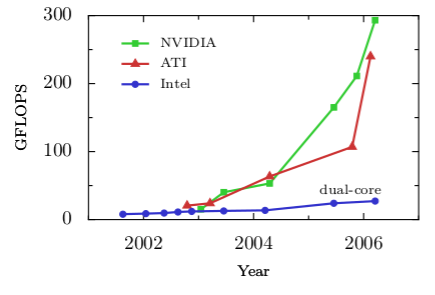
\includegraphics[width=0.6\textwidth]{figuras/cpuGpu2006.png}
%     \source{\cite{owens2007survey}}
%     \caption{Evolução do desempenho entre GPUs (verde e vermelho), contra
%     CPUs (azul), dentre os anos 2000 e 2006.}
%     \label{fig:cpuGpu2006}
% \end{figure}

%    \textit{survey} \cite{owens2007survey}
%
% 	Uma das primeira aplicações envolvendo o uso de GPUs no processamento de imagens foi feito por
% \cite{fung2005openvidia}, que descreve o arcabouço de programação \textit{OpenVIDIA}, criado a partir do
% \textit{OpenGL}, desenvolvido por \cite{opengl}. Antes do \textit{OpenVIDIA} o processamento de imagens em GPUs era
% feito utilizando o \textit{OpenGL}, uma linguagem para processamento gráfico, voltada para a renderização de cenas. Os
% algoritmos para processamento de imagem eram reescritos para utilizarem primitivas do \textit{OpenGL}. O
% \textit{OpenVIDIA} criou um encapsulamento de chamadas do \textit{OpenGL} voltado para imagens, retirando a necessidade
% de traduzir os algoritmos e facilitando a utilização dos \textit{shaders} programáveis da GPU.
%
% 	Com a introdução de linguagens próprias para programação em GPU, vários algoritmos de processamento de imagens foram
% traduzidos para a execução em GPUs. Na área de registro um dos primeiros artigos a tratar do assunto foi
% \cite{strzodka2004image}, que apresenta uma implementação de um algoritmo de registro não-rígido que utiliza uma técnica
% de redução de energia da diferença das imagens. \cite{kohn2006gpu} expandiu o trabalho anterior, criando uma versão do
% algoritmo para imagens em três dimensões e realizando um registro rígido antes do não-rígido. Ainda programando
% diretamente em \textit{OpenGL}, \cite{vetter2007non} propõem um algoritmo de registro multimodal para imagens médicas
% executando em uma GPU 7800 da \textit{NVIDIA}. O artigo leva em conta a organização da imagem na memória da GPU e o
% tempo de transmissão dos dados da CPU para a GPU.
%
% 	O trabalho de \cite{grossauer2008gpu} relata a criação de um algoritmo para registro que utiliza fluxo óptico em
% conjunto com métodos de \textit{Multi Grid}, usados para resolver equações diferenciais parciais. Ele descreve
% a aceleração do \textit{Multi Grid}, dada a sua afinidade com o \textit{Pipeline} gráfico. Em \cite{bui2009performance}
% o passo de interpolação de um algoritmo de registro multi modal entre imagens médicas é traduzido utilizando uma
% linguagem para programação genérica em GPUs, o CUDA \cite{nvidia2007compute}. O estudo realiza uma comparação de
% eficiência entre o código em CPU e GPU de uma interpolação bilinear, apresentando como resultado uma aceleração de 60
% vezes da GPU em relação a CPU. O algoritmo de registro proposto por \cite{han2009gpu} utiliza Informação Mutua para
% realizar um registro não-rígido entre imagens de ressonância magnética entre cérebros de indivíduos e um atlas com a
% finalidade de segmentar regiões de interesse no individuo. O estudo utiliza uma GPU \textit{NVIDIA} em conjunto com a
% linguagem CUDA para registrar as imagens, apresentando uma aceleração de 25 vezes em relação a CPU. Esse estudo,
% juntamente com o anterior, se preocupa com a organização dos dados na memória da GPU, algo que era de dificil controle
% antes do surgimento de linguagens voltadas para GPGPU.
%
% 	Em 2010, o artigo de \cite{modat2010fast} define um algoritmo de registro não-rígido chamado de \textit{Free-Form
% Deformation}, desenvolvido para registrar imagens de ressonância magnética pesadas em T1. Diferente de outros algoritmos,
% ele foi desenvolvido para executar em GPUs diretamente. Para tal, os autores utilizam uma interpolação B-Spline cúbica e
% uma modificação da informação mutua como métrica para o registro. Ele separa cara passo em vários \textit{kernels} diferentes, fazendo
% com que cada \textit{kernel} utilize o máximo de memória possível e então espalha o processamento para um maior número
% de processadores na GPU, melhorando o desempenho do algoritmo.
%
% 	O estudo de \cite{membarth2011frameworks} realiza uma comparação entre vários arcabouços de programação para GPU,
% entre eles o CUDA e o OpenCL utilizando como caso de comparação o registro de imagens 2D/3D, ou seja, o registro de
% imagens em três dimensões de tomografia computadorizada para imagens de raio-X. O artigo então segue primeiro com uma
% comparação conceitual entre os vários arcabouços e depois com uma comparação de desempenho. Foram feitas comparações
% com a execução sequencial, em paralelo e em GPU do algoritmo.

%% ------------------------------------------------------------------------- %%
\section{Objetivos}

  Vários trabalhos na última década estudam o mapeamento de algoritmos de
registro para GPUs. Normalmente, só o mapeamento dos métodos é apresentado, sem
explorar recursos encontrados nas placas gráficas que podem ser aplicados para
aumentar o desempenho da implementação. Dentre tais recursos estão a utilização
a execução concorrente de vários kernels ou a utilização de texturas
tridimensionais.

  O principal objetivo do trabalho é apresentar uma implementação do Thin Plate
Splines em GPU, aperfeiçoado para a execução de $n$ instâncias de registro, onde
cada instância registra uma imagem alvo diferente para a mesma imagem referência.
Nossa implementação será separada em blocos, que podem ser executados tanto em
CPU quanto em GPU, a escolha do usuário. Os objetivos específicos deste
trabalho são:

\begin{enumerate}
	\item Explorar soluções para incrementar o desempenho na execução do registro
        de várias imagens alvo para a mesma imagem referência
	\item Identificar quais melhorias de desempenho características da GPU podem
        ser aplicadas no mapeamento do TPS
	\item Desenvolver uma implementação configurável, que possa ser executada
        em ambientes GPU ou CPU
  \item Estudo comparativo entre as melhorias aplicadas
\end{enumerate}

%% ------------------------------------------------------------------------- %%
\section{Organização do Trabalho}
\label{sec:organizacao_trabalho}

No Capítulo~\ref{cap:conceitos}, os conceitos utilizados pelo trabalho
são apresentados, como registro e GPGPU. O capítulo \ref{cap:metodologia}
mostra como os conceitos são combinados para a criação da implementação que
satisfaz nossos objetivos. No Capítulo \ref{cap:resultados} os experimentos são
descritos e os seus resultados avaliados. Finalmente, no Capítulo
~\ref{cap:conclusoes} analisamos os resultados obtidos.
